\chapter{Evaluation and discussion}\label{chapter:evaluation}

This chapter evaluates the performance of the automatically generated translation. I compare runtimes of various versions of the same functions. I compare the original function against its translation. I measure the effect of the presented optimizations and compare the translation against a manually optimized formulation.

Plots are drawn using logarithmic x- and y-axis to depict the large differences in runtimes. Additionally, polynomial growth is easier to differentiate from exponential growth when using logscales. A polynomial function on a xy-logscale appears as a straight line, the slope determines the degree of the polynomial. A linear function, ie. a polynomial of degree 1, has a slope of 1.

\paragraph*{Evaluation setup}
The evaluations were run on a system running Ubuntu 18.04.1 with 4.15 Linux-Kernel, AMD 1900X with 8x 3.80GHz (16 Threads), 256MB NVMe SSD and 16GB DDR4 RAM. PostgreSQL 10.6 on default settings, if not stated otherwise.

The call stack of PostgreSQL is limited in size to prevent infinite recursion from quickly sucking up the entire system memory. The default in PostgreSQL 10.6 (\texttt{max\_stack\_depth}) is 2MB and can manually be increased. The maximum stack size is capped by the settings of the Operating System.\\
The available working memory (\texttt{work\_mem}) specifies how much memory can be consumed by in-memory operations like sorting or hashing. If the memory is exceeded temporary results are materialized on disk. The default working memory is 2MB. \cite[p. 512 ff.]{psql}

To fully exploit the capabilities of each implementation the \texttt{max\_stack\_size} is set to 7680kB (the limit of the OS) and the working memory (\texttt{work\_mem}) to 512MB. This way recursive functions can run longer before being killed. The high working memory enables operations like sorting or hashing to be performed in memory, even for larger inputs.

The original recursive functions were run until the stack size was exceeded and the function was killed. The translations were run (where possible) at least as long as the original function until the trend of the curves seems to be clear.

To track plans and times of parts of the translation the extension \texttt{auto\_explain} was used with \texttt{log\_nested\_statements}, \texttt{log\_verbose} and \texttt{log\_timing} enabled. Logging format (\texttt{log\_format}) was set to JSON.

\section{Generic Template}

The generic template is the default template without any UDF-specific optimizations as presented in \autoref{template}. The performance of the Fibonacci function (\autoref{intro_fib}) from the introduction is shown in \autoref{fig:fib_times}.

\begin{figure}[h!]
    \centering\small
    \includesvg{plots/fib}
    \caption{Run time of the Fibonacci function in its recursive version and the automatic translation. Additionally, a manually optimized version is compared.}
    \label{fig:fib_times}
\end{figure}

Runtimes vary greatly between the three implementations. The original implementation is faster for very small inputs as it has less overhead then the translation. Additionally, the first two (\texttt{fib(\$1-1)} and \texttt{fib(\$1-2)}) calls are inlined which reduces overhead further. However, the runtime of the original function grows very fast, \texttt{fib(30)} already takes minutes.

The translated function is much faster nonetheless. Where the original takes minutes the translation is finished under 10ms. Even for \texttt{fib(1000)} the call returns after about 2 seconds. For very small inputs the runtime seems to be nearly constant, possibly because the tiny computations are marginalized by the constant overhead of the template. After leveling up the runtime of the translation has a slope of approximately 2 indicating quadratically growth.

Nevertheless, the translation cannot keep up with the manually optimized function. The step from the translation to the manually optimized version is similar in magnitude to the step from the original to the translation: The runtime drops from minutes to milliseconds.\\
Though the runtime grows as the inputs get even larger, but in a slower pace. The implementation provided runs nearly in linear time exploiting the need of only two values to be remembered to compute the next value.\\

Eventually, other limitations stop computing even larger Fibonacci numbers in PostgreSQL: Somewhere between fib(600000) and fib(700000) the numeric datatype (which can represent numbers up to 131072 digits! \cite[p. 124 f.]{psql}) fails with an overflow. That being said, the manual optimized implementation is "as good as we can get" in SQL.

Each implementation has changed the complexity-class of the implementation. The recursive implementation of \texttt{fib} is exponential as previously computed values are repeatedly recomputed. Actually, the calltrees of the callsites are identical except for a single call.

Problems with overlapping subproblems, as with Fibonacci, are subject to an optimization technique called "Dynamic Programming" and "Memoization". Starting from optimal subproblems solutions of larger problems are incremental computed. Dynamic Programming requires therefore to reformulate the algorithm to implement this approach. Memoization solves the problem top-down keeping the original recursive structure of the function. It is checked for each call whether this call was already evaluated. If so, the saved value is returned. Our translation uses the original recursive formulation and applies automatic memoization avoiding any redundant calls.

If an algorithm has no overlapping subproblems and there are no redundant calls memoization gives no speedup. Each calltree of the callsites is disjunct. The evaluation of these algorithms grounds on recursively dividing the problem in disjunct subproblems. The results then are recursively merged to construct the final result ("divide and conquer"). An example with two callsites is \texttt{quicksort} (\autoref{udf:quicksort}).

\begin{figure}[h!]
    \centering\small
    \includesvg{plots/nonoverlapping}
    \caption{Runtimes for quicksort as a quadratic divide and conquer algorithm.}
    \label{fig:nonoverlapping_times}
\end{figure}

\autoref{fig:nonoverlapping_times} shows that the translation still causes a speedup roughly by factor 10 for \texttt{quicksort}. This is remarkable because the function does not profit from memoization. This plot illustrates boldly how PostgreSQL is highly optimized for efficient operations on tables and not for efficient function calls.

As a last aspect of the generic translation I examine the fraction of time spent in each part of the translation \autoref{fig:split_times}. We see that the evaluation is by far the costliest part of the translation. Noteworthy is the large fraction the bare result selection takes. This can be explained by the following: Each iteration of the evaluation works on a linear growing working-table which is together with the new results appended to the final result. The final result of the CTE includes lots of duplicates which are only seen when selecting the result. Therefore both parts constantly have a significant influence on the total runtime, opposed to callgraph and basecase which marginalize over time.

\begin{figure}[h!]
    \centering\small
    \includesvg{plots/split}
    \caption{Percentage of runtime for each part of the translation of \texttt{fib}}
    \label{fig:split_times}
\end{figure}


\iffalse
\begin{figure}[h]
    \centering\small
    \includesvg{plots/recN}
    \caption{Impact of the number of scenarios on the runtime. Single recursive function with expensive predicates}
    \label{fig:recn_times}
\end{figure}

Impact of number of scenarios (Overhead by predicates) \autoref{fig:recn_times}

\fi




\section{Single and Tail Recursion}

Functions with only one callsite per scenario are called \textit{single recursive functions}. In the context of this thesis I rank them among the group of divide and conquer algorithms as they have no overlapping subproblems. Consecutively, I use the \texttt{sum} (\autoref{udf:sum}) function as an example to study the performance of the translation.

\begin{figure}[h!]
    \centering\small
    \includesvg{plots/sum}
    \caption{Sum as example for a single recursive function. Calls to the original \texttt{sum} eventually exceed stack depth.}
    \label{fig:factorial_times}
\end{figure}


Surprisingly, the generic translation of \texttt{sum} yields a runtime even worse than the original quicksort function. Quicksort was run with an array of descending numbers thus the runtime equals the worst case of $O(n^2)$. The original single recursive version of \texttt{sum} grows roughly linear as we can see from the plot. The generic translation of \texttt{sum} degrades the performance of the linear function heavily. It is even worse than quicksort (\autoref{fig:nonoverlapping_times}) -- which is quadratic.

\autoref{fig:split_sr_times} depicts the fraction of time each part of the translation consumes from the total computation time for a given input. On the left, the data is taken from the badly performing generic translation. On the right, the translation using the single recursive optimization is shown. Noticeably, the generic translation evaluation marginalizes all other parts of the translation.

\begin{figure}[h!]
    \centering\small
    \includesvg{plots/split_sr}
    \caption{Fraction of total runtime spend in each part of the translation of \texttt{sum}.}
    \label{fig:split_sr_times}
\end{figure}

This slowdown is apparently caused by the growth of the evaluation CTE. All previous results are accumulated there and each result adds all previous results to allow access to results from all earlier iterations. This behaviour makes the evaluation-CTE grow quadratically, even if the original function is linear.

But this does not explain why the function performs worse than the quadratic non-memoizable quicksort. The problem is caused by the wrong guess of the query planner about the number of rows returned from the scan of \texttt{callgraph}. During scenario-evaluation the CTE \texttt{e} (proxying \texttt{evaluation}) is joined with \texttt{callgraph} two times: Once for joining callsites with their results using a hash join ($O(n+m)$, good). The other join is caused by the \texttt{NOT EXISTS} which is rewritten into a \texttt{LEFT JOIN}.

\begin{figure}[h!]
    \centering\scriptsize
    \begin{verbatim}
->  Nested Loop Anti Join  (cost=0.00..20.54 rows=1 width=68) (actual time=0.118..15.206 rows=250 loops=500)
	Output: c_3.in_1, c_3.call_site, c_3.out_1
	Join Filter: (e_1.in_1 = c_3.in_1)
	Rows Removed by Join Filter: 83333
	->  CTE Scan on callgraph c_3  (cost=0.00..4.29 rows=1 width=68) (actual time=0.000..0.077 rows=499 loops=500)
	    Output: c_3.in_1, c_3.call_site, c_3.out_1
	    Filter: (c_3.call_site = ANY ('{1}'::integer[]))
	    Rows Removed by Filter: 1
	->  CTE Scan on e e_1  (cost=0.00..10.00 rows=500 width=32) (actual time=0.000..0.011 rows=168 loops=249500)
	    Output: e_1.in_1, e_1.res
    \end{verbatim}
    \caption{Extract of the query plan of scenario evaluation from \texttt{sum(500)}, translated using the generic template.}
    \label{plan:sum}
\end{figure}

The planner assumes that only a single row is returned from \texttt{callgraph} after filtering with \texttt{c.callsite\_id IN (1)} and therefore chooses to make a \textit{nested loop anti join}. Nested loop joins are a good choice if one table is small because the runtime is $O(nm)$ \cite{???}. But the UDF has only a single callsite. Accordingly, the predicate is not selective at all and not one but all $n$ rows are returned. The working-table of evaluation has a size of $n/2$ on average. Thus the join complexity is in $O(n^2)$ -- for a single iteration. 

Evaluation of the callgraph happens in a level-wise fashion, one level per iteration. Recalling \autoref{???} the callgraph of a single recursive function is just a linked list so the depth of the callgraph is $n$. For quicksort the callgraph is a binary tree hence the depth is just $log_2(n)$. In sum, the generic translation of a single recursive functions increases complexity from $O(n)$ to $O(n^3)$.

Using the template for single recursion fixes this issue. The template does not accumulate all previous results in the current result thus the working-table does not grow with $n$, but always yields only a single row. The size of \texttt{evaluation} remains linear.

The original function starts out linear but slows down a bit for large inputs before exceeding stack size. The speedup by the optimized translation is roughly by factor 10 with no limitation by the maximum stack size.

The tail recursive optimization speeds up performance constantly by the factor of approx. 2. This seems natural considering that \autoref{fig:split_sr_times} shows the evaluation-CTE, which is omitted in the tail recursive template, accounting for approx. 40\% of the runtime.

\section{Template Optimizations}


\begin{figure}[h!]
    \centering\small
    \includesvg{plots/paramN_opts}
    \caption{Impact of the different optimizations, compared to the original function \texttt{param4} (see \autoref{udfs:paramN})}
    \label{fig:paramN}
\end{figure}



\autoref{fig:paramN} looks surprising. The original functions all perform similar and much better than the translations. Even more interesting: The UDF with just one argument performs worst. This behaviour is surprising since one would assume a simpler function to perform better in the translation because there is less data to manage and hence joining tables is easier.\\
A first explanation could be the additional arguments giving the functions more selective join predicates. Yet, this cannot be the case as the additional arguments of the used functions are just the arguments passed to the function ergo the values are equal for all calls.\\
A possible reason for the big difference lies in the join order of the evaluation-subqueries since the query plan reveals \autoref{???}. The function with one argument and n=200 at first makes a nested loop anti-join join \texttt{evaluation} (rows=500, actual=68) with \texttt{callgraph} (rows=1, actual=201). The result (rows=1, actual=100) is joined with a hash join with \texttt{evaluation} (rows=500, actual=101).\\
The UDF with four arguments has flipped the order of the joins: First, a hash join between \texttt{evaluation} (rows=940, actual=102) and \texttt{callgraph} (rows=100, actual=201) happens. The result (rows=1, actual=101) is joined with a nested loop anti-join with \texttt{evaluation} (rows=940, actual=69).

Nested Loop Joins are a good choice when one table is small. Otherwise a hash join performs better. The other plan uses a hash join first and then the nested loop join. As a result, the nested loop join is executed on a smaller table which explains the better run-time. The plan from the UDF with one argument performs a nested loop join on tables with 68 and 201 rows while for the other plan the inputs are sized 69 and 101 rows.

Now to the observation that the original performs better than the translation. This can be explained by the property of the given function being linear recursive. No branching occurs and no memoization can be exploited. The overhead of the translation is significant is such a case: The evaluation-CTE adds all the previous results to the new result for each step. The number of rows is therefore $(0 + 1) + (1 + 1) + (2 + 1) + \dots + (n + 1) = \frac{n(n+1)}{2}$ thus in $O(n^2)$. With the translation we have made a linear function quadratic. Note that the results were obtained with optimizations disabled. Hence there is hope as we see in the next section comparing optimizations to their originals.


% When limiting stack size to 100kb, param1_tr(320) is the first argument where it dies with "stack depth limit exceeded". As the function is nearly as simple as it gets, is seems to be valid to assume as lower bound that SQL will consume 1/3 kB per layer on the callstack. With default OS settings of max of 8MB on my machine, this means a maximum recursion depth of not more than roughly 25000 layers.  


\begin{figure}
    \centering
    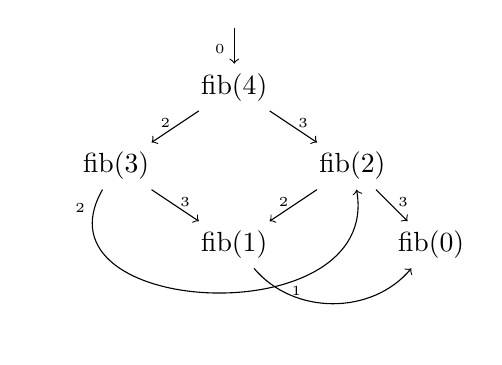
\begin{tikzpicture}
% nodes
\node (f4)     at (2.5, 2) {fib(4)};
    \node (f3) at (1, 1) {fib(3)};
        \node (f1) at (2.5, 0) {fib(1)};
    \node (f2) at (4, 1) {fib(2)};
        \node (f0) at (5, 0) {fib(0)};
% arrows
\draw[<-] (f4) -- node[pos=0.4, left, label distance=5mm]{\tiny{0}} +(0, 0.75);

\draw[->] (f4) -- node[pos=0.4, left, label distance=5mm]{\tiny{2}} (f3);
\draw[->] (f4) -- node[pos=0.4, right, label distance=5mm]{\tiny{3}} (f2);

    \draw[->, bend right=100, out=240, looseness=1.5] (f3) to node[pos=0.05, left, label distance=5mm]{\tiny{2}} (f2);
    \draw[->] (f3) -- node[pos=0.4, right, label distance=5mm]{\tiny{3}} (f1);
    \draw[->] (f2) -- node[pos=0.4, left, label distance=5mm]{\tiny{2}} (f1);
        \draw[->, bend right=50] (f1) to node[pos=0.2, right, label distance=5mm]{\tiny{1}} (f0);
    \draw[->] (f2) -- node[pos=0.4, right, label distance=5mm]{\tiny{3}} (f0);
\end{tikzpicture}
    \caption{Callgraph with memoization, The callstack-tree becomes a Directed Acyclic Graph (DAG). Each node represents an invocation and each outgoing edge a new callsite. Because of memoization evaluation of equal invocations is performed only once, ie. they have the same descendants.}
    \label{fig:fib_callstack_memoization}
\end{figure}



\section{Future work}

This thesis provides only a first working version of the general approach developed by the Database Systems Research Group at Tübingen. Naturally, there are many topics for future work.

\subsection{Template optimization}
The template is already highly optimized but still there is room for improvements. There are some "low-hanging fruits" and some topics that need further research.

\paragraph*{Evaluation of predicate-parts in own CTE}
Currently, predicates are created during scenario analysis. Each predicate duplicates all the previous predicates by including them negated. If each part is evaluated once in a CTE and then just referenced in further predicates this redundant evaluations can be eliminated. Queries with costly predicates and many scenarios would profit from this small change.\\
This could happen either in a post-processing step of the predicates or the predicate in the rules is replaced with an supporting data-structure.

\paragraph*{\texttt{LIMIT}s}
In the evaluation we have seen how wrong guesses have led the query planner to serious misconceptions impacting runtime severely. By adding explicit \texttt{LIMIT}s to subqueries we give the planner explicit information about how many rows to expect. Furthermore, expensive joins can be stopped as soon as the first and only row has been returned. For example the single recursive template will always just return a single row per iteration of the evaluation-CTE. Therefore scenario evaluation can be stopped after the single row is returned.\\
The same is applicable for final result collection: Instead of doing a \texttt{DISTINCT} a \texttt{LIMIT 1} would have the same effect. There definitely are further possibilities to add explicit \texttt{LIMIT <n>} statements, maybe from an analysis of the callgraph.

\paragraph*{Nullable arguments}
Currently, only UDFs can be translated with non-\texttt{NULL} arguments. Joining tables with \texttt{=} yields false when comparing \texttt{NULL}-values. Yet, \texttt{NULL} can be an valid input. \texttt{IS NOT DISTINCT FROM} does consider two \texttt{NULL}s as equal, but the join-performance is heavily impacted as experiments have shown. This is reasonable since the join-predicate \texttt{x IS NOT DISTINCT FROM y} is just syntactic sugar for \texttt{x = y OR (x IS NULL AND y IS NULL)}.

The solution may be to distinguish between \texttt{STRICT} and \texttt{NON STRICT} UDFs. Functions tagged as \texttt{STRICT} are functions that return \texttt{NULL} straight away if any of their arguments is \texttt{NULL}. The actual function is not evaluated in this case. Therefore no call with a \texttt{NULL} argument will lead to subsequent callsites hence all recursive scenarios have non-\texttt{NULL} arguments. Calls with a \texttt{NULL}-argument are thus only required to be considered when collecting basecases. During evaluation all arguments are not nullable and \texttt{=} can be used safely. Argument-comparisons for \texttt{NON STRICT} UDFs would fallback to use \texttt{IS NOT DISTINCT FROM}.

\subsection{Extend applicability}

The current translation template does not work for every possible recursive UDF. It would be great if some of the constraints could be lifted in the future to widen applicability of our approach.

\paragraph*{Allow row-variables in predicates and arguments}
This is the constraint that limits the real world usage of the translation the most. SQL is made for operations on tabular data but the translation barely supports this yet. The challenge is to extract an evaluable fragment of code from an arbitrary position in an arbitrarily nested query. The fragment must be evaluated for every possible value of its row-reference. In this manner the callgraph gets a new dimension: A scenario is evaluable if all callsites have results for every row available. Surely, there are a number of other complexities and challenges which must be solved first.

\paragraph*{Allow dependant callsites}
Another constraint is callsites not being allowed to depend on each other. Recursive function arguments like $f(f(n-1))$ are not allowed as the argument must be evaluated in advance to create the callgraph. The Ackermann function is a prominent example for such a function.

Another form of dependency between callsites is of two recursive predicates at the same level. This is unfortunate since any form of backtracking algorithm uses this pattern: If a recursive call with current arguments fails then backtrack recursively. The recursive call in the predicate would cause the scenario analysis to return the entire fragment as a single scenario.\\
This limitation may be lifted with an iterative partial construction of the callgraph.

\paragraph*{Translation from and to other languages}

The UDF-slices from the scenario analysis could be used to fill templates in another target language, eg. PL/SQL or C. The general idea from the translation could also be applied to other languages.

\subsection{Optimize evaluation}

The callgraph is a precious source of information about the runtime-behaviour of the recursive function. If we can exploit this information evaluation can happen much more efficiently.

Problematic about the workaround allowing back-references in self-referential CTEs is the accumulation of lots of redundant rows. These duplicates cannot be removed from the growing result of the CTE during evaluation and need to be eventually traversed in order to select the result of the evaluation.

Another option is to use the callgraph to read only those rows which are required by later callsites. In each iteration of the evaluation, one topological level of the callgraph is evaluated. It is easy to check after each iteration which nodes in the callgraph have no more dependencies to callsites which are not already evaluated. Those values can be safely removed from the result set as these results will not be needed again.

Yet another possibility is to analyze the maximum dependency distance to include only the last $n$ results in every iterations result. For the Fibonacci-function such a analysis would limit the size of the working table constantly to 2. This approach could give a great speedup for many problems and would be easy to implement.

Furthermore, we could analyze the callgraph and annotate points of interest. It may be beneficial to prune the evaluation table periodically or at advantageous points, eg. when a large subtree is completely evaluated. Pruning could happen by restarting evaluation, keeping only required rows.

Another option is to persist tables in an unlogged temporary table. This has the advantage of rows being easily to remove if not required anymore. This could happen as a periodical side-effect during translation. Further, tables could be indexed and different processes could parallelly work together. Especially divide and conquere algorithms could benefit as they only need few evaluation passes and produce a large number of disjunct calls.\\
Persisted tables could also be used to memoize calls not only from the current query, but also from earlier queries. This could be used to implement a caching mechanism.

Analyzing the callgraph may reveal independent subtrees which could be evaluated in parallel. This could either happen by manually triggering parallel execution by starting own processes that access common tables or by utilizing PostgreSQLs own parallel-query capabilities. 